% % % % % % % % % % % % % % % % % % % % % % % % % % % % % % % % % % % % % % % % 
% Formelsammlung von LaTeX4EI									
%
% @encode: 	UTF-8, tabwidth = 4, newline = LF
% @author:	Emanuel Regnath
% @date:		
%
% % % % % % % % % % % % % % % % % % % % % % % % % % % % % % % % % % % % % % % % 


%---------------------------------------%
%			P R E A M B L E				%
%~~~~~~~~~~~~~~~~~~~~~~~~~~~~~~~~~~~~~~~%

% Document Class ===============================================================
\documentclass[fs, footer]{latex4ei}

\usepackage{multirow}			% Spaltenpaket

\usepackage{tikz}				% Alle möglichen Zeichnungen

\sisetup{per-mode = fraction}

%---------------------------------------%
%			Kommunikationsnetze 			%
%~~~~~~~~~~~~~~~~~~~~~~~~~~~~~~~~~~~~~~~%

% DOCUMENT_BEGIN ===============================================================
\begin{document}

% Split in 4 Columns ===========================================================
\begin{multicols*}{4}





% TITLE ========================================================================
\fstitle{Kommunikationsnetze}

\section*{Allgemeines}

\sectionbox{
	\begin{center}
		\Fbox{Quelle} $\ra$ \Fbox{Sender} $\ra$ \Fbox{Kanal} $\ra$ \Fbox{Empfänger} $\ra$ \Fbox{Senke}\\[1em]
	\end{center}

	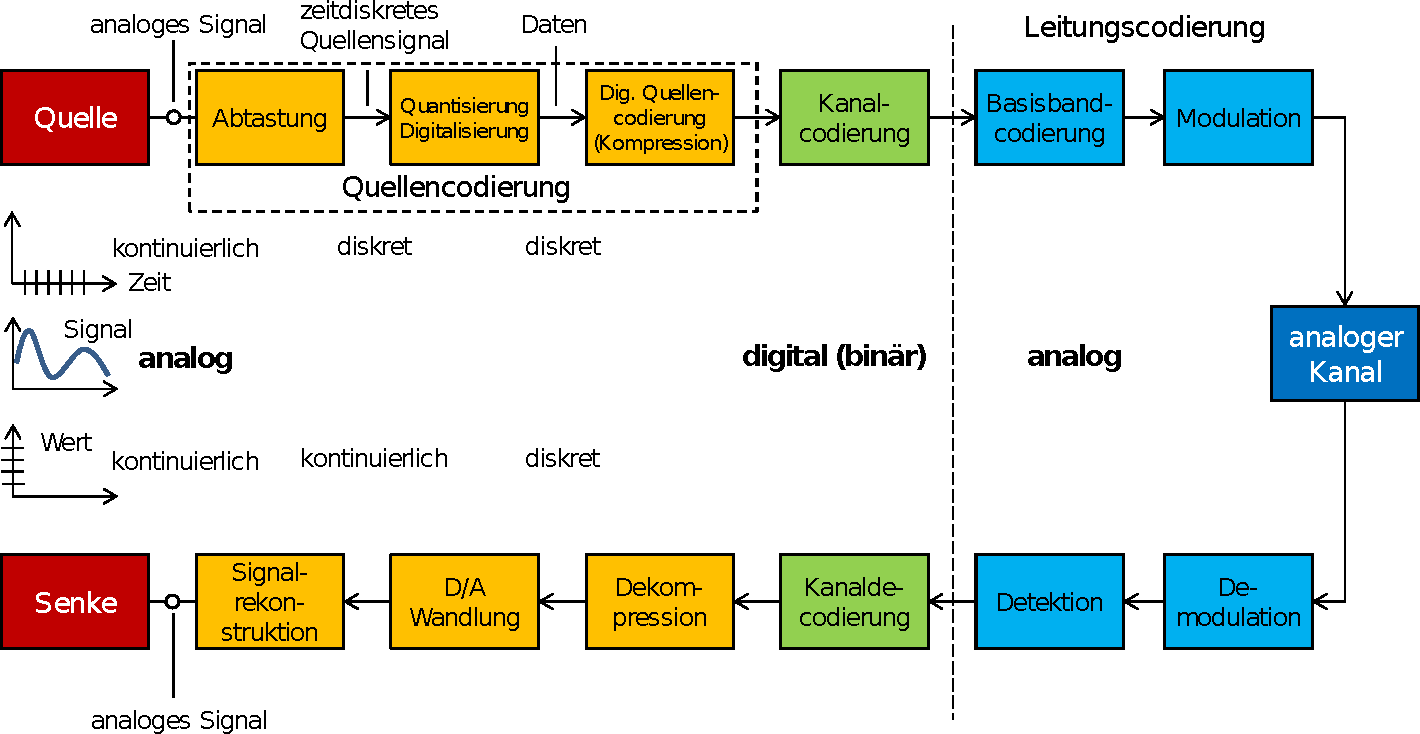
\includegraphics[width = \columnwidth]{./img/transmission.pdf}

}







% SECTION ====================================================================================
\section{Signale}
\sectionbox{
	\subsection{Arten von Signalen}
	\begin{description}
		\item[deterministisch:] durch Funktionen beschreibbar, enthalten kein Nachricht.
		\item[stochastisch:] zufälliger Verlauf, überträgt Information
	\end{description}
	
	
	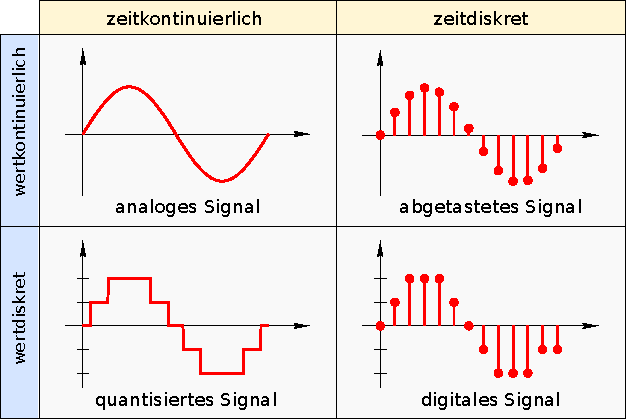
\includegraphics[width = \columnwidth]{./img/signals.pdf}

	Vorteile digitales Signal: Kompression, Verschlüsselung, Fehlerkorrektur
}


\sectionbox{
	\subsection{Abtasttheorem}	
	Signal muss bandbegrenzt sein. \\ 

	\emphbox{
	Abtasttheorem nach Shannon \quad $f_{\ir a} \ge 2 f_{\ir S_{\ir max}}$
	}
}





% SECTION ====================================================================================
\section{Nachrichtenaustausch}

\sectionbox{
	 \symbolbox{
	\begin{tabular}{cc}
	 $T_S$ &  Sendedauer \\
	 $T_P$ & Übertragungsdauer (Signal Propagation) \\
	 $T_{V_i}$ & Verzögerungszeit im Knoten
	\end{tabular}
	 }

	 Übertragungsdauer: $T_P = \frac{l}{c_{\ir Kanal}}$ \\

	Sendedauer: $T_S = \frac{L}{R}$
	%\begin{tabular}{lll}
	 %& Circuit Switching & Packet Switching \\
	%& Leitungsvermittlung & Paketvermittlung\\
	%& (volle Belegung der Ressourcen) &  (Paket-Multiplex Gewinn)\\
	%connection & Ende-zu-Ende Verbindung \\
	% orientented &  & Ende-zu-Ende Verbindung aufbauen, in jedem NE: Pakete folgen einem festgelegten Weg, logische Verbindung \\
	%connectionless & nicht möglich & in jedem NE: Zieldaten, die jedes Paket tragen muss werden ausgewertet
	%\end{tabular}
}





% SECTION ====================================================================================
\section{Verkehrstheorie} 

\sectionbox{
	\subsection{Zufallsverkehr} 

	Poisson Prozess: $p_k (t) = \frac{t^k \lambda^k}{k!} \exp (- \lambda t)$

}

\sectionbox{
	\subsection{Wartesystem M/M/N/$\infty$}
	\symbolbox{
		\begin{tabular}{cc}
			$P_W$ & Wartewahrscheinlichkeit \\
			$\Omega$ & durchn. Warteschlangenlänge \\
			$T_W$ & durchschnittl. Wartezeit \\
			$T_D$ & durchsch. Durchlaufzeit
		\end{tabular}

	} \\ \\
	Druchlaufzeit: $T_D = T_W + h$



	Zustandswahrscheinlichkeit: $P_x = P_0 \prod \limits^x_{i = 1} \frac{\lambda_{i-1}}{\mu_i}$

	$\epsilon = \frac{1}{h}$ \quad $\lambda = \frac{1}{a}$


	Angebot: $A = \frac{\lambda}{\epsilon} = \lambda \cdot h$


	Sterberate $\mu_x = \begin{cases}
	x\epsilon & \text{für } x = 1, 2, \ldots, N \\ N \epsilon & x = N, N+1, \ldots \infty
	\end{cases}$ \\

	Zustandsverteilung:

	$p_x = \begin{cases}
	p_0 \frac{A^x}{x!} & \text{für } x = 0,1 , \ldots, N \\ p_0 \frac{A^N}{N!} (\frac{A}{N})^{x-N} & \text{für } x = N, N+1, \ldots, \infty
	\end{cases}$ \\ \\

	Wartewahrscheinlichkeit:

	$P_W = \sum \limits_{i=0}^{\infty} P_n (\frac{A}{N})^i = P_N \frac{N}{N-A} = \frac{\frac{A^i}{N!} \frac{N}{N-A}}{\sum \limits_{i = 0}^{N-1} \frac{A^i}{i!} + \frac{A^N}{N!} \frac{N}{N-A}}$ \\

	mittlere Warteschlangenlänge:

	$\Omega = \sum \limits^{\infty}_{x = N} (x - N) P_x = P_N \cdot \rho \frac{1}{(1- \rho)^2} = P_N \frac{\frac{A}{N}}{(1 - \frac{A}{N})^2}$ \\ \\

	mittlere Wartezeit (Gesetz von Little) : $T_W = \frac{\Omega}{\lambda}$ \\ 



	\subsubsection{Sonderfall M/M/1/$\infty$}

	Wartewahrscheinlichkeit $P_W |_{N =1} = A$

	Warteschlangenlänge: $\Omega |_{N=1} = \frac{\rho}{1 - \rho}$

	Wartezeit: $T_W = \frac{\rho}{\lambda (1 - \rho)}$
}

\sectionbox{
	\subsection{Verlustsystem M/M/N/-}

	Zustandsverteilung: $p_x = \frac{\frac{A^x}{x!}}{\sum \limits_{k=0}^N \frac{A^k}{k!}}$ mit $x = 0, 1, 2, \ldots N$

	Verlustwahrscheinlichkeit (Blockierung): $B = p N = \frac{\frac{A^N}{N!} }{\sum \limits_{k=0}^N \frac{A^k}{k!}}$
}


\section{Protokolle}

\subsection{ARQ Quittungsprotokoll}


\symbolbox{
	\begin{tabular}{cc}
	 $p_M$ & Wahrscheinlichkeit das Message verloren geht \\
	 $p_A$ & Wahrscheinlchkeit das ACK verloren geht 
	\end{tabular}
} 

Wahrscheinlichkeit für korrekte Übertragung (ACK und Message): $p_S = (1 - p_M) (1 - p_A)$

Fehlerwahrscheinlichkeit: $p_E= 1 - p_S$

Mittelwert der Zahl der Sendeversuche pro $M$: $s = \frac{1}{1 - p_E}$

$r = s - 1$

$T_T = T_A + 2 (T_p + T_V)$

Wirkungsgrad $\rho = \frac{T_S}{rT^* + T_S + T_A + 2 (T_P + T_V)}$


Optimale Paketlänge  $L_{\ir opt} \aprox \sqrt{\frac{2R(T_P + T_V)}{p_B}} $


% Ende der Spalten
\end{multicols*}

% Dokumentende
% ======================================================================
\end{document}